% !TEX root = ../main.tex
% File: chapters_part1/chap3_4.tex
% Nội dung cho Phần 3.4: Seq2Seq và Attention

\section{Mô hình Chuỗi-sang-Chuỗi (Seq2Seq) và Cơ chế Chú ý (Attention)}
\label{sec:seq2seq_attention}

Kiến trúc RNN, LSTM, hay GRU mà chúng ta vừa học có một hạn chế cơ bản: chúng được thiết kế để xử lý các bài toán có đầu vào là một chuỗi và đầu ra là một giá trị duy nhất (phân loại) hoặc một chuỗi có độ dài bằng với chuỗi đầu vào (gán nhãn chuỗi).

Nhưng điều gì sẽ xảy ra với các bài toán như \textbf{dịch máy} (một câu tiếng Việt có 10 từ có thể được dịch thành một câu tiếng Anh 8 từ) hoặc \textbf{tóm tắt văn bản} (một văn bản 1000 từ được tóm tắt thành một câu 20 từ)? Ở những bài toán này, độ dài chuỗi đầu vào và đầu ra là khác nhau và không có sự tương ứng 1-1.

Mô hình Chuỗi-sang-Chuỗi (Sequence-to-Sequence - Seq2Seq) ra đời để giải quyết chính xác vấn đề này.

\subsection{Kiến trúc Encoder-Decoder của Seq2Seq}
\label{ssec:encoder_decoder}
Seq2Seq, được giới thiệu gần như đồng thời bởi Sutskever và các cộng sự (2014) \cite{sutskever2014sequence} và Cho và các cộng sự (2014) \cite{cho2014learning}, dựa trên một kiến trúc thanh lịch gồm hai thành phần chính: \textbf{Bộ mã hóa (Encoder)} và \textbf{Bộ giải mã (Decoder)}.

\begin{center}
    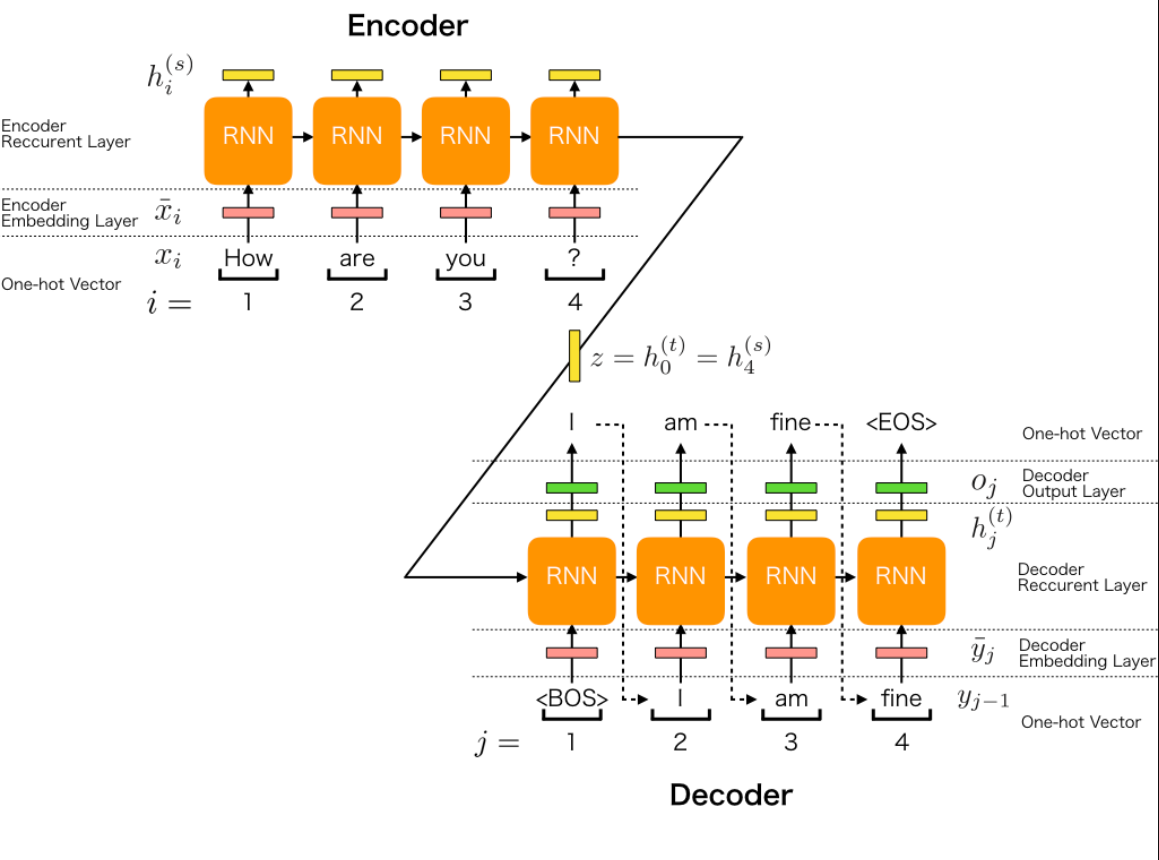
\includegraphics[width=0.9\textwidth]{seq2seq_architecture.png}
    \captionof{figure}{Kiến trúc Encoder-Decoder tổng quát. Encoder "đọc" và nén chuỗi đầu vào thành một vector ngữ cảnh. Decoder sử dụng vector này để "viết" ra chuỗi đầu ra.}
    \label{fig:seq2seq_architecture}
\end{center}

\subsubsection{Bộ mã hóa (The Encoder)}
\paragraph{Nhiệm vụ}
Nhiệm vụ của Encoder là "đọc" toàn bộ chuỗi đầu vào (ví dụ, một câu tiếng Việt) và nén toàn bộ thông tin, ngữ nghĩa của nó vào một vector có kích thước cố định. Vector này được gọi là \textbf{vector ngữ cảnh (context vector)} hay "thought vector".

\paragraph{Cấu tạo và Hoạt động}
\begin{itemize}
    \item Encoder thường là một mạng RNN (hoặc LSTM, GRU).
    \item Nó nhận đầu vào là một chuỗi các vector từ (word embeddings) của câu nguồn, ví dụ: $x_1, x_2, \dots, x_T$.
    \item Nó xử lý chuỗi này tuần tự, từng từ một. Tại mỗi bước, nó cập nhật trạng thái ẩn của mình.
    \item Điều quan trọng là chúng ta \textbf{bỏ qua tất cả các đầu ra (outputs) của Encoder ở mỗi bước}. Chúng ta chỉ quan tâm đến \textbf{trạng thái ẩn cuối cùng ($h_T$)}. Trạng thái ẩn cuối cùng này chính là vector ngữ cảnh, vì nó được cho là đã tóm tắt thông tin của toàn bộ chuỗi đầu vào.
\end{itemize}
\begin{tcolorbox}[
    title=Ghi chú sâu về Thiết kế của Encoder,
    colback=green!5!white, colframe=green!50!black, fonttitle=\bfseries
]
\textbf{1. Tại sao Encoder thường là Mạng RNN Hai chiều (Bi-RNN)?} \\
Một RNN đơn giản xử lý câu từ trái sang phải. Trạng thái ẩn $h_t$ tại từ $x_t$ chỉ chứa thông tin về các từ từ $x_1$ đến $x_t$. Điều này là một hạn chế, vì ngữ nghĩa của một từ thường phụ thuộc vào cả ngữ cảnh đứng trước và đứng sau nó.
\begin{itemize}
    \item \textbf{Bi-RNN} giải quyết vấn đề này bằng cách sử dụng hai RNN riêng biệt: một RNN chạy xuôi (forward) từ đầu đến cuối câu, và một RNN chạy ngược (backward) từ cuối về đầu.
    \item Tại mỗi từ $x_t$, biểu diễn cuối cùng của nó là sự \textbf{kết hợp} (thường là nối - concatenation) của trạng thái ẩn từ cả hai chiều: $\overrightarrow{h_t}$ và $\overleftarrow{h_t}$.
    \item Vector ngữ cảnh cuối cùng cho mô hình Seq2Seq cơ bản sẽ là nối của trạng thái ẩn cuối cùng của RNN xuôi ($\overrightarrow{h_T}$) và trạng thái ẩn cuối cùng của RNN ngược ($\overleftarrow{h_1}$).
\end{itemize}
Việc này cung cấp một biểu diễn ngữ cảnh phong phú hơn nhiều cho mỗi từ, và đã trở thành tiêu chuẩn trong hầu hết các mô hình Encoder-Decoder.

\textbf{2. Tại sao không dùng Pooling thay vì trạng thái ẩn cuối cùng?} \\
Sử dụng trạng thái ẩn cuối cùng là cách đơn giản nhất, nhưng nó có thể bị ảnh hưởng bởi "hiệu ứng gần đây" (recency bias) - các từ cuối chuỗi có thể có ảnh hưởng lớn hơn. Các phương pháp khác như:
\begin{itemize}
    \item \textbf{Average/Max Pooling:} Lấy trung bình hoặc giá trị lớn nhất trên tất cả các trạng thái ẩn (của Bi-RNN). Cách này dân chủ hơn, đảm bảo mọi từ đều có đóng góp, nhưng có thể làm "lu mờ" các chi tiết quan trọng.
\end{itemize}
Trong thực tế, trước khi Attention ra đời, không có phương pháp nào là hoàn hảo. Sự ra đời của Attention đã giải quyết triệt để vấn đề này bằng cách cho phép Decoder tự quyết định nên tập trung vào đâu, thay vì ép Encoder phải tạo ra một bản tóm tắt duy nhất.
\end{tcolorbox}
\subsubsection{Bộ giải mã (The Decoder)}
\paragraph{Nhiệm vụ}
Nhiệm vụ của Decoder là lấy vector ngữ cảnh do Encoder cung cấp và "giải nén" nó để sinh ra chuỗi đầu ra (ví dụ, câu tiếng Anh tương ứng), từng từ một.

\paragraph{Cấu tạo và Hoạt động}
\begin{itemize}
    \item Decoder cũng là một mạng RNN (hoặc LSTM, GRU) khác, thường có kiến trúc tương tự Encoder nhưng với bộ trọng số riêng.
    \item \textbf{Khởi tạo:} Trạng thái ẩn ban đầu của Decoder ($h_0^{dec}$) được khởi tạo bằng chính vector ngữ cảnh (trạng thái ẩn cuối cùng của Encoder, $h_T^{enc}$). Đây là "cây cầu" duy nhất kết nối Encoder và Decoder.
    \item \textbf{Quá trình sinh từ (Generation):} Quá trình này diễn ra tuần tự:
        \begin{enumerate}
            \item \textbf{Bước 1:} Decoder nhận vào một token bắt đầu đặc biệt (ví dụ: `<SOS>` - Start of Sentence) và trạng thái ẩn ban đầu. Nó tính toán trạng thái ẩn mới $h_1^{dec}$ và tạo ra một phân phối xác suất trên toàn bộ từ vựng của ngôn ngữ đích thông qua một lớp softmax. Từ có xác suất cao nhất được chọn làm từ đầu ra đầu tiên, $y_1$.
            \item \textbf{Bước 2:} Từ vừa được sinh ra, $y_1$, sẽ trở thành \textbf{đầu vào cho bước tiếp theo}. Decoder nhận $y_1$ và trạng thái ẩn $h_1^{dec}$ để tính $h_2^{dec}$ và sinh ra từ tiếp theo $y_2$.
            \item Quá trình này lặp đi lặp lại (mang tính \textbf{tự hồi quy - auto-regressive}) cho đến khi Decoder sinh ra một token kết thúc đặc biệt (`<EOS>` - End of Sentence).
        \end{enumerate}
\end{itemize}

\subsubsection{Vấn đề của cái "Cổ chai" (The Bottleneck Problem)}
Kiến trúc Encoder-Decoder cơ bản này rất thông minh, nhưng nó có một điểm yếu chết người: nó buộc Encoder phải nén toàn bộ thông tin của một câu, dù dài và phức tạp đến đâu, vào một \textbf{vector ngữ cảnh có kích thước cố định}.
\begin{itemize}
    \item Đây là một "cổ chai" thông tin. Với những câu dài, việc nhồi nhét tất cả các chi tiết ngữ nghĩa vào một vector duy nhất là cực kỳ khó khăn, nếu không muốn nói là bất khả thi.
    \item Decoder chỉ được "nhìn" vào bản tóm tắt này một lần duy nhất lúc bắt đầu. Nó không có cách nào để quay lại và xem xét các phần cụ thể của câu nguồn khi nó đang dịch.
\end{itemize}
Hãy tưởng tượng bạn yêu cầu một dịch giả nghe toàn bộ một bài phát biểu dài, sau đó phải dịch lại toàn bộ từ trí nhớ mà không được ghi chép. Đó chính là những gì mô hình Seq2Seq cơ bản phải làm. Hạn chế này đã dẫn đến sự ra đời của ý tưởng có sức ảnh hưởng bậc nhất trong lịch sử NLP hiện đại: \textbf{Cơ chế Chú ý (Attention)}.

\subsubsection{Huấn luyện mô hình Seq2Seq}
Mục tiêu huấn luyện của mô hình Seq2Seq là tối đa hóa xác suất của chuỗi đầu ra đúng ($Y = y_1, ..., y_{T'}$) khi biết chuỗi đầu vào ($X = x_1, ..., x_T$). Điều này tương đương với việc tối thiểu hóa hàm mất mát \textbf{Cross-Entropy} trên toàn bộ chuỗi đầu ra:
$$ \mathcal{L}(\theta) = - \sum_{t=1}^{T'} \log P(y_t | y_1, ..., y_{t-1}, c) $$
trong đó $c$ là vector ngữ cảnh từ Encoder. Trong quá trình huấn luyện, lỗi tại mỗi bước của Decoder được tính toán và lan truyền ngược qua cả Decoder và Encoder để cập nhật tất cả các trọng số. Kỹ thuật \textbf{Teacher Forcing} được sử dụng để làm cho quá trình này ổn định và hiệu quả hơn.

\subsubsection{Huấn luyện và Suy luận: Teacher Forcing và Beam Search}
Có hai kỹ thuật quan trọng liên quan đến cách mô hình Seq2Seq được huấn luyện và sử dụng để sinh văn bản.

\paragraph{Huấn luyện với Teacher Forcing}
Trong quá trình huấn luyện, tại mỗi bước $t$, thay vì đưa từ mà Decoder vừa dự đoán ở bước $t-1$ vào làm đầu vào, chúng ta lại đưa từ \textbf{chính xác (ground truth)} trong chuỗi đích vào.
\begin{itemize}
    \item \textbf{Ưu điểm:} Kỹ thuật này giúp quá trình huấn luyện ổn định và hội tụ nhanh hơn rất nhiều. Nó ngăn ngừa việc lỗi bị tích tụ: nếu mô hình dự đoán sai ở bước đầu, lỗi sai đó sẽ không làm ảnh hưởng đến các bước sau trong cùng một chuỗi huấn luyện. Mỗi bước thời gian được coi là một mẫu huấn luyện độc lập.
    \item \textbf{Nhược điểm:} Nó tạo ra một sự khác biệt giữa lúc huấn luyện và lúc suy luận (khi mô hình không có "thầy" để chỉ bảo). Điều này có thể dẫn đến hiệu năng kém khi mô hình phải tự sinh ra một chuỗi dài.
\end{itemize}

\paragraph{Suy luận với Beam Search}
Trong lúc suy luận, việc luôn chọn từ có xác suất cao nhất tại mỗi bước (gọi là \textbf{Greedy Search}) thường không tạo ra được câu tốt nhất. Một lựa chọn có vẻ tốt ở hiện tại có thể dẫn đến một ngõ cụt. \textbf{Beam Search} là một giải pháp cân bằng.
\begin{itemize}
    \item Thay vì chỉ giữ lại 1 ứng viên tốt nhất ở mỗi bước, Beam Search sẽ giữ lại $k$ ứng viên (gọi là \textit{beam width} hoặc \textit{kích thước beam}) có xác suất chuỗi cao nhất.
    \item Tại bước tiếp theo, nó sẽ mở rộng mỗi ứng viên trong beam với tất cả các từ khả dĩ trong từ vựng, tính toán xác suất của các chuỗi mới, và lại chọn ra $k$ chuỗi tốt nhất để tiếp tục.
    \item Quá trình này là một sự đánh đổi giữa chất lượng và chi phí tính toán. Nó hiệu quả hơn nhiều so với Greedy Search và là kỹ thuật tiêu chuẩn để sinh văn bản trong các mô hình Seq2Seq.
\end{itemize}
\subsection{Cơ chế Chú ý (Attention Mechanism)}
\label{ssec:attention}

\subsubsection{Trực giác cốt lõi: Dịch như con người}
Khi một dịch giả con người dịch một câu, họ không làm như mô hình Seq2Seq cơ bản. Khi dịch một từ, họ sẽ tập trung (pay attention) vào một hoặc một vài từ liên quan trong câu gốc. Cơ chế Chú ý được thiết kế để mô phỏng chính xác hành vi này.

\begin{tcolorbox}[
    title=Ý tưởng đột phá của Attention,
    colback=yellow!10!white, colframe=yellow!50!black, fonttitle=\bfseries
]
Thay vì ép Encoder tạo ra một vector ngữ cảnh duy nhất, hãy cho phép Decoder, tại \textbf{mỗi bước} sinh từ của mình, có khả năng \textbf{"nhìn lại" toàn bộ chuỗi đầu vào} và quyết định xem phần nào của chuỗi đầu vào là quan trọng nhất cần phải "chú ý" đến ngay tại thời điểm đó.
\end{tcolorbox}

Attention tạo ra một "đường tắt" kết nối trực tiếp Decoder với tất cả các trạng thái ẩn của Encoder, phá vỡ cái "cổ chai" thông tin.

\subsubsection{Cơ chế hoạt động chi tiết}
Cơ chế chú ý được tích hợp vào giữa Encoder và Decoder. Thay vì chỉ truyền trạng thái ẩn cuối cùng, Encoder sẽ cung cấp \textbf{tất cả các trạng thái ẩn của nó} ($h_1^{enc}, h_2^{enc}, \dots, h_T^{enc}$) cho Decoder.

Bây giờ, tại mỗi bước $t$ của Decoder, để sinh ra từ $y_t$, nó sẽ thực hiện các bước sau:

\begin{center}
    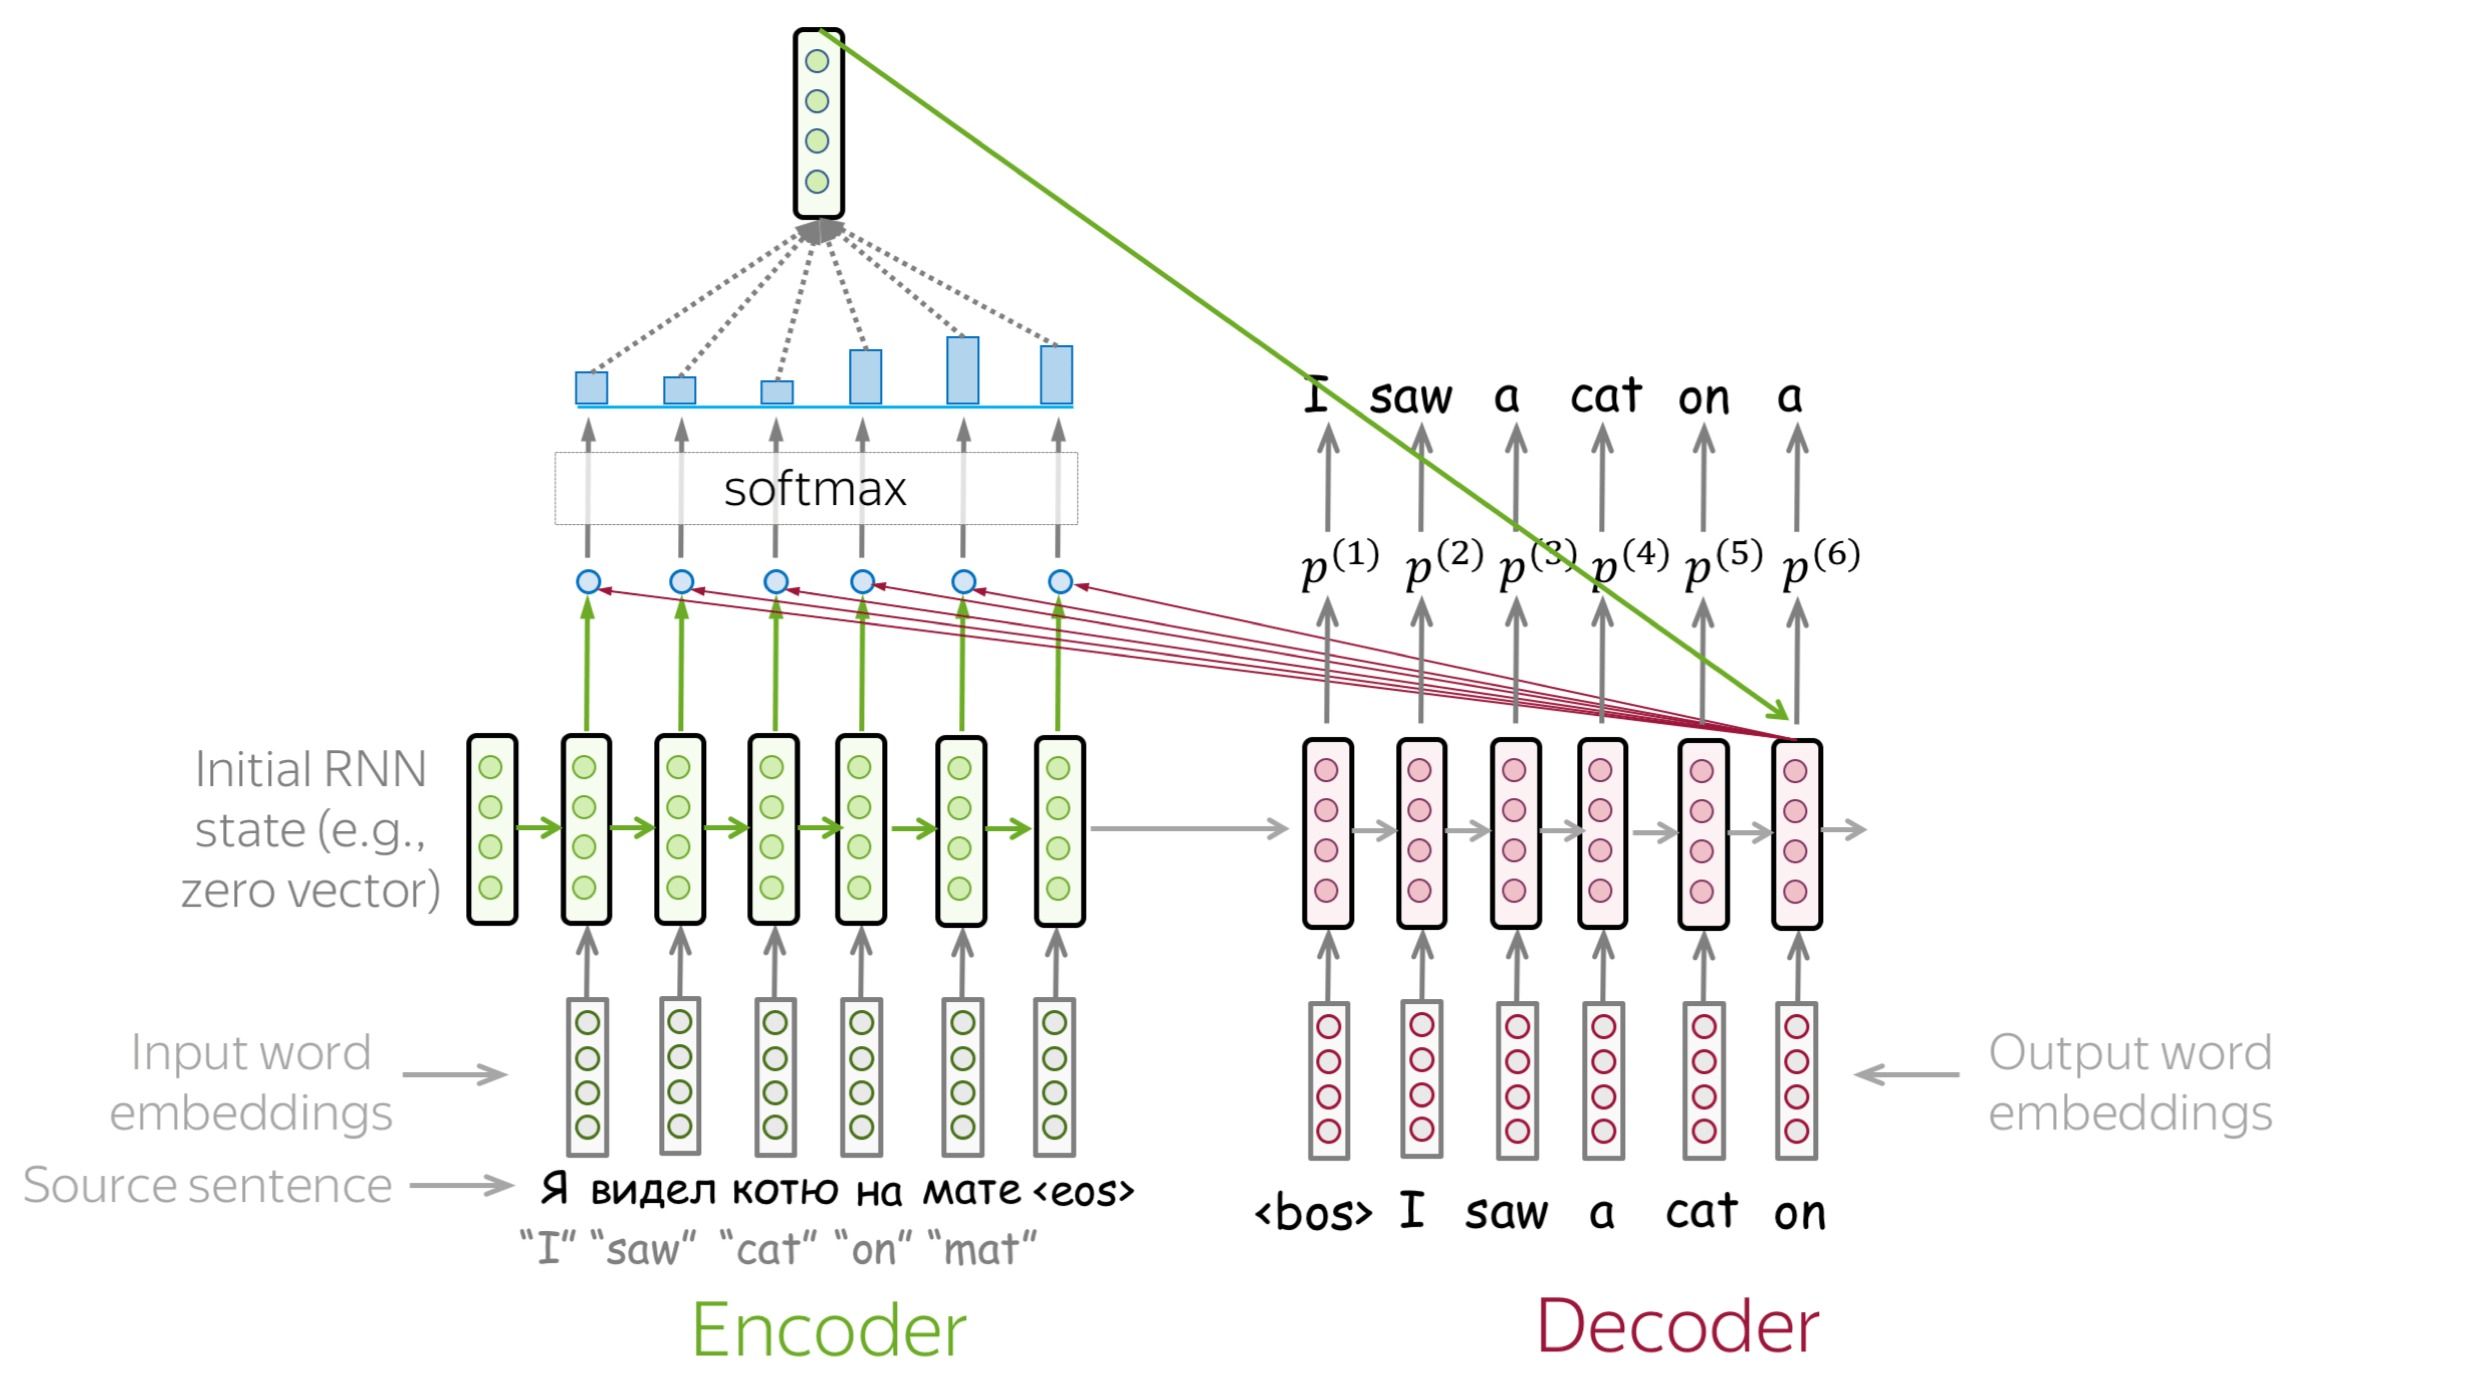
\includegraphics[width=1.0\textwidth]{seq2seq_attention_mechanism.png}
    \captionof{figure}{Cơ chế Chú ý trong Seq2Seq. Tại bước sinh từ thứ $t$ của Decoder, nó tính toán các trọng số chú ý ($\alpha_t$) để tạo ra một vector ngữ cảnh động ($c_t$) từ tất cả các trạng thái ẩn của Encoder.}
    \label{fig:seq2seq_attention_mechanism}
\end{center}

\paragraph{Bước 1: Tính điểm chú ý (Attention Scores)}
Decoder lấy trạng thái ẩn của nó ở bước trước, $h_{t-1}^{dec}$, và so sánh nó với \textbf{từng trạng thái ẩn của Encoder}, $h_i^{enc}$, để tính ra một "điểm số tương hợp" (alignment score). Điểm số này đo lường mức độ "liên quan" của từ đầu vào thứ $i$ đối với việc sinh ra từ đầu ra thứ $t$. Có nhiều cách để định nghĩa hàm $\text{score}(h_{t-1}^{dec}, h_i^{enc})$, trong đó phổ biến là:
\begin{itemize}
    \item \textbf{Additive Attention (\cite{bahdanau2014neural}):} Sử dụng một mạng nơ-ron nhỏ truyền thẳng (feed-forward) có một lớp ẩn. Cách này mạnh mẽ và linh hoạt.
        $$ \text{score}(h_{t-1}^{dec}, h_i^{enc}) = v_a^T \tanh(W_a [h_{t-1}^{dec}; h_i^{enc}]) $$
    \item \textbf{Dot-Product Attention (\cite{luong2015effective}):} Đơn giản là lấy tích vô hướng giữa hai vector. Cách này rất nhanh và hiệu quả về mặt tính toán, nhưng yêu cầu số chiều của $h^{dec}$ và $h^{enc}$ phải bằng nhau.
        $$ \text{score}(h_{t-1}^{dec}, h_i^{enc}) = (h_{t-1}^{dec})^T h_i^{enc} $$
    \item \textbf{Scaled Dot-Product Attention:} Một biến thể của Dot-Product, được giới thiệu trong bài báo Transformer \cite{vaswani2017attention}. Nó chia tích vô hướng cho căn bậc hai của số chiều vector ($\sqrt{d_k}$) để tránh gradient quá nhỏ khi số chiều lớn.
\end{itemize}
Sự lựa chọn hàm score ảnh hưởng đến độ phức tạp tính toán và hiệu năng của mô hình. Dot-Product và các biến thể của nó đã trở nên rất phổ biến do hiệu quả của chúng, đặc biệt là trong kiến trúc Transformer.
\paragraph{Bước 2: Chuẩn hóa thành trọng số (Softmax)}
Các điểm số vừa tính được sẽ được đưa qua một hàm \textbf{softmax}. Điều này biến các điểm số thành một phân phối xác suất, gọi là \textbf{trọng số chú ý (attention weights)}, ký hiệu là $\alpha_{ti}$.
$$ \alpha_{ti} = \frac{\exp(\text{score}(h_{t-1}^{dec}, h_i^{enc}))}{\sum_{j=1}^{T} \exp(\text{score}(h_{t-1}^{dec}, h_j^{enc}))} $$
Tổng của tất cả các trọng số $\alpha_{ti}$ (với $i$ từ 1 đến $T$) bằng 1. Mỗi $\alpha_{ti}$ cho biết "mức độ chú ý" mà Decoder nên dành cho từ đầu vào thứ $i$ khi sinh ra từ đầu ra thứ $t$.

\paragraph{Bước 3: Tính toán vector ngữ cảnh động (Context Vector)}
Vector ngữ cảnh $c_t$ bây giờ không còn cố định nữa. Nó là một \textbf{tổng có trọng số (weighted sum)} của tất cả các trạng thái ẩn của Encoder, với các trọng số chính là các trọng số chú ý vừa tính được.
$$ c_t = \sum_{i=1}^{T} \alpha_{ti} h_i^{enc} $$
Vector ngữ cảnh $c_t$ này được tính toán lại ở \textbf{mỗi bước của Decoder}. Nếu các trọng số chú ý $\alpha_{ti}$ tập trung vào trạng thái ẩn thứ $j$ của Encoder, thì vector $c_t$ sẽ chủ yếu chứa thông tin từ $h_j^{enc}$.

\paragraph{Bước 4: Sử dụng vector ngữ cảnh để dự đoán}
Cuối cùng, vector ngữ cảnh động $c_t$ được nối với trạng thái ẩn của Decoder ở bước trước, $h_{t-1}^{dec}$, và được đưa vào làm đầu vào cho lớp RNN của Decoder để tính ra trạng thái ẩn hiện tại $h_t^{dec}$.
$$ h_t^{dec} = \text{RNN}_{\text{dec}}(h_{t-1}^{dec}, c_t) $$
Trạng thái $h_t^{dec}$ này sau đó được dùng để dự đoán từ đầu ra $y_t$. Một cách khác là nối $c_t$ với $h_t^{dec}$ trước khi đưa vào lớp softmax cuối cùng.

\subsubsection{Sức mạnh của Attention}
\begin{itemize}
    \item \textbf{Phá vỡ nút thắt cổ chai:} Thông tin không còn bị nén vào một vector duy nhất. Decoder có quyền truy cập vào toàn bộ chuỗi đầu vào ở mọi thời điểm.
    \item \textbf{Khả năng diễn giải (Interpretability):} Chúng ta có thể trực quan hóa ma trận trọng số chú ý để xem mô hình đang "nhìn" vào đâu khi dịch. Ví dụ, khi dịch từ "bạn", mô hình sẽ có trọng số chú ý cao nhất ở từ "you". Điều này giúp gỡ lỗi và hiểu mô hình tốt hơn.
    \item \textbf{Hiệu năng vượt trội:} Các mô hình Seq2Seq với Attention đã ngay lập tức thiết lập một tiêu chuẩn mới về chất lượng cho dịch máy và nhiều bài toán chuỗi-sang-chuỗi khác, vượt xa các hệ thống thống kê trước đó.
\end{itemize}

Cơ chế Chú ý không chỉ là một cải tiến. Nó là một trong những ý tưởng nền tảng và có sức ảnh hưởng lớn nhất trong lịch sử học sâu, là tiền đề trực tiếp cho sự ra đời của kiến trúc Transformer mà chúng ta sẽ tìm hiểu ở chương tiếp theo.